\documentclass[letterpaper]{article} % DO NOT CHANGE THIS
\usepackage[submission]{aaai2027}  % DO NOT CHANGE THIS
\usepackage[hyphens]{url}  % DO NOT CHANGE THIS
\usepackage{graphicx} % DO NOT CHANGE THIS
\urlstyle{rm} % DO NOT CHANGE THIS
\def\UrlFont{\rm}  % DO NOT CHANGE THIS
\usepackage{natbib}  % DO NOT CHANGE THIS AND DO NOT ADD ANY OPTIONS TO IT
\usepackage{caption} % DO NOT CHANGE THIS AND DO NOT ADD ANY OPTIONS TO IT
\frenchspacing  % DO NOT CHANGE THIS

% Permitted additions (not on the forbidden list)
\usepackage{amsmath,amssymb,amsthm}
\usepackage{booktabs}
\usepackage{tikz}
\usetikzlibrary{arrows.meta,positioning}

\pdfinfo{
/TemplateVersion (2027.1)
}

\setcounter{secnumdepth}{0}

% ---------- Convenience ----------
% Figure include that compiles even before the real PDFs are dropped in.
% Put the four generated PDFs in a figures/ directory next to this file.
\newcommand{\figorbox}[2]{%
  \IfFileExists{#1}{\includegraphics[width=#2]{#1}}{%
    \fbox{\parbox[c][1.6in][c]{\dimexpr#2-2\fboxsep-2\fboxrule\relax}{\centering
      \texttt{\detokenize{#1}}\\(drop generated PDF here)}}}}

\newtheorem{proposition}{Proposition}

% ---------- Title ----------
% TODO(Nathan): pick one. Mixed case required by AAAI.
% Option A (mechanism-forward):
\title{Only Destruction Survives: Honest Evaluation of Attribute Removal in Learned Representations}
% Option B (law-forward):
% \title{Outputs Leak What They Use: Certificates, Costs, and the Floor of Attribute Removal}
% Option C (sober):
% \title{Attribute Removal Under Honest Evaluation: A Characterization, a Diagnostic, and a Method}

\author{Anonymous submission}
\affiliations{ }

\begin{document}

\maketitle

\begin{abstract}
% TODO(Nathan): rewrite in your voice. Structure to keep:
% (1) problem: removal methods are certified with weak probes;
% (2) re-audit finding: 3 of 21 verdicts survive honest probing; hiding fails;
% (3) the law + diagnostic (upper bound, r=0.795);
% (4) the method: shape-then-destroy, near-zero representation-side cost,
%     only the output-level floor remains (wall INSIDE the claim);
% (5) gauntlet: 1 of 36 published-method combinations certifies, including
%     NeurIPS'25 code failing on its authors' own probe.
Methods that remove a protected attribute from a learned representation are routinely certified with weak probes. We re-audit such certificates under a strong attacker battery and find that only 3 of 21 previously ``stopped'' verdicts survive. Across projection, adversarial scrubbing, and sealed-channel designs, erasure shaped against a probe fools only that probe. We characterize why: task outputs leak whatever information they actually use, so output-side leakage is bounded below by a floor set by the label--attribute coupling, which a one-feature test predicts in advance (Pearson $r=0.795$; the predictor is an upper bound that is tight when the task is well learned). We propose a training procedure that concentrates attribute information into a designated subspace and destroys it, removing representation-side leakage at near-zero utility cost and leaving only the output-level floor, which we show is fundamental. Certification depends on attacker knowledge: against black-box attackers our method certifies at 85--102\% retained utility, while informed attackers with clean-data side information are stopped only by full-rank noise at substantial cost. Under identical two-tier evaluation, 1 of 36 published-baseline combinations certifies, and the one survivor does so through incidental sampling noise rather than its fairness mechanism.
\end{abstract}

\section{Introduction}
% DRAFT BELOW (Claude): rewrite everything in your voice.
% Claim-shape rules that must survive your rewrite:
%  - never a bare utility number; the wall rides inside every headline
%  - "linear certificates, though deliberately scoped, leave a large nonlinear
%    gap that practical evaluations rarely check; we quantify it"
%  - hard cell: "85+/-2% at the 0.55 bar (90% at a relaxed 0.57 bar)"
%  - no coined terms; "approaching the leakage floor established by
%    \citet{stadler2024}" not "leak-optimality"

Machine learning systems are increasingly required to make predictions without exposing protected attributes such as race or sex. A large body of work answers this requirement at the level of the representation: train or transform an encoder so that the attribute can no longer be recovered from it, then certify compliance by probing the representation and reporting that recovery is at chance. The certificate is only as strong as the probe. In practice the probe is almost always weak, a linear model or the method's own adversary, and the guarantee inherits that weakness silently.

This paper asks what happens to such certificates under honest evaluation, and what honest protection actually costs. We assemble a strong attacker battery, gradient-boosted trees, deep probes, low-rank adaptation probes, and an informed likelihood-ratio attacker with clean-data side information, and re-audit compliance verdicts that weak certificates had granted. The result is stark. Of 21 verdicts in which a weak certificate reported an attribute ``stopped,'' 3 survive the battery. The failures are not close: representations certified at near-zero linear recoverability routinely yield the attribute to a tree-based probe at AUC above 0.9. Linear certificates, though deliberately scoped to linear adversaries \citep{belrose2023leace}, leave a nonlinear gap that practical evaluations rarely check. We quantify that gap, and we find it is the rule rather than the exception.

The failures share a mechanism. Every method we audit that attempts to \emph{hide} attribute information, orthogonal projections, kernel-statistic penalties, adversarial scrubbing, sealed architectural channels, fails against attackers it was not shaped against, because the information is still present. The only mechanism that survives is \emph{destruction}: adding noise that removes the information outright. This is not an artifact of our implementations. Under identical two-tier evaluation, published baselines fail the same way on their authors' own code, and the single published method that certifies anywhere does so through the sampling noise its variational objective happens to inject, not through its fairness machinery.

Honest destruction has a price, and the price obeys a law. Task outputs leak whatever information they actually use, so when a task genuinely depends on an attribute, the model's decisions reveal it regardless of how thoroughly the representation is scrubbed. We measure this floor across tabular and vision cells and find it tracks the label--attribute coupling along the diagonal. The coupling is measurable in advance by a one-feature probe of the labels alone, giving a diagnostic that predicts the utility cost of honest removal before any training run (Pearson $r=0.795$ across 20 natural cells, confirmed causally on constructed cells). The diagnostic is an upper bound on output leakage. It is tight when the task is well learned and loose otherwise, a boundary we establish by falsifying our own prediction on a vision cell and reconciling the miss.

Within the regime the law permits, removal can be made nearly free. We propose a training procedure that shapes the representation to concentrate attribute information into a designated subspace and then destroys that subspace with noise. Ablations show both halves are necessary: shaping without destruction leaks, destruction without shaping pays full-rank prices. Against black-box attackers the procedure certifies at 102\%, 100\%, and $85\pm2$\% retained utility on our three headline cells at a 0.55 recovery bar (90\% at a relaxed 0.57 bar), removing representation-side leakage at near-zero cost and leaving only the output-level floor, which is fundamental. Certification is relative to attacker knowledge: an informed attacker that knows the channel and the clean-data statistics defeats every subspace-targeted defense by reading the noise-free complement, and is stopped only by full-rank noise at substantial utility cost. Protection, we find, must be priced by threat tier.

Our contributions:
\begin{itemize}
    \item \textbf{An honest re-audit.} Under a strong two-tier attacker battery, 3 of 21 weak-certificate verdicts survive; probe-shaped erasure fools only the matching probe (Fig.~\ref{fig:demolition}).
    \item \textbf{Two propositions.} Linear certificates are provably invariant under linear downstream adaptation, so their apparent stability against linear attack is vacuous (Prop.~\ref{prop:blind}); and no certificate computed from second-moment statistics can be non-vacuous at practical operating points (Prop.~\ref{prop:impossible}). Together they imply adversarial empirical evaluation is not optional.
    \item \textbf{A law and a diagnostic.} Output-side leakage is floored by label--attribute coupling (Fig.~\ref{fig:diagonal}); a one-feature test predicts removal cost in advance, as an upper bound with a measured validity condition (Fig.~\ref{fig:ramp}).
    \item \textbf{A method reaching the floor.} Shape-then-destroy training removes representation-side leakage at near-zero cost at Tier~1 and characterizes the full price of Tier~2 (Fig.~\ref{fig:twotier}).
    \item \textbf{A provenance-audited gauntlet.} 1 of 36 published-baseline combinations certifies under identical evaluation, on official code where it exists (Table~\ref{tab:gauntlet}).
\end{itemize}

\section{Related Work}
% TODO(Nathan): tighten to ~0.6pp. The five risk papers, each cited first by us,
% differences stated at true size, confidently:
% - \citet{stadler2024}: proved a fundamental leakage floor exists. We provide the
%   empirical characterization, the a-priori predictor, causal confirmation, and a
%   method that approaches the floor. (Foundation, not competitor.)
% - \citet{zhao2019inherent}: information-theoretic fairness-utility tradeoffs; our
%   cost ramp is the measured face of that tension.
% - \citet{ravfogel2022kernelized}: showed erasure does not transfer across adversary
%   classes; we quantify how large the gap is in practice, systematically.
% - \citet{jovanovic2023fare}: certified fair representations against restricted
%   downstream models; our evaluation is strong-attacker and empirical.
% - Probing-methodology critiques (MDL probing, amnesic probing): the evaluation-
%   standard ancestry \citep{voita2020mdl,elazar2021amnesic}.
% Plus: overlearning \citep{song2020overlearning}; convergent evidence from
% diffusion-model erasure \citep{lu2025erasure}; TAR/RMU durability failures as
% motivation \citep{tamirisa2024tar,qi2024durability}.
% Field-claim calibration sentence lives here too.
[Related work stub: five risk papers thrown at ourselves first, at true size.]

\section{Setup: Cells, Battery, and Why Measurement Must Be Adversarial}

We evaluate on three headline tabular cells, named by their label-coupling
difficulty throughout: \textbf{easy} (HMDA, race $\to$ loan\_decision,
predictor $0.514$), \textbf{middle} (HMDA, race $\to$ loan\_amount\_band,
$0.584$), and \textbf{hard} (Adult, sex $\to$ income, $0.603$), plus two
CelebA vision cells selected by the same statistic. Difficulty here is an
output-side property, set by how strongly the label couples with the
attribute, not a representation-side one: every clean representation we
test leaks its attribute at essentially $1.0$, so representation-side
intuition orders these cells identically and wrongly. Attribute recovery
is measured as macro one-vs-rest AUC, where $0.5$ is chance and $0.55$ is
the protection bar. The recovery battery has two tiers, priced by attacker
knowledge. Tier~1 is black box: XGBoost \citep{chen2016xgboost}, a deep MLP
(256--256), and a rank-32 ReLU LoRA probe \citep{hu2022lora}. Tier~2 adds a
channel-aware Gaussian likelihood-ratio attacker that knows the clean
representation and the noise law. The LoRA member is not redundant: in the
end-to-end experiments it breached configurations that XGBoost and the MLP
both passed, so a battery without it would have certified operating points
that do not hold. Certified operating points are the mean over three
training seeds with the full battery on the representation and on the task
outputs, and every headline point is re-run at five seeds. In plain terms,
a method is only credited with hiding an attribute if the strongest probe
we can build, at the stated knowledge tier, reads near chance on every
exposed surface.

\begin{proposition}[Linear certificates are blind to linear adaptation]
\label{prop:blind}
% TODO(Nathan): final statement wording with Raff. Content: linear R^2 (and
% dominant-axis R^2) between a representation and an attribute is invariant under
% any invertible affine map of the representation; hence no strictly linear
% downstream adapter can change a linear certificate's reading.
Let $h \in \mathbb{R}^d$ be a representation and $z$ an attribute. For any invertible affine map $A$, the linear coefficient of determination satisfies $R^2_{\mathrm{lin}}(Ah, z) = R^2_{\mathrm{lin}}(h, z)$. Consequently a linear certificate cannot register any strictly linear downstream adaptation, and its stability under linear attack carries no evidential weight.
\end{proposition}

\begin{proposition}[Second-moment certificates are vacuous]
\label{prop:impossible}
% TODO(Nathan): scope precisely with Raff. Content: for any certificate computed
% from second-moment statistics of the noised representation, there exist
% distributions matching those statistics on which an attacker achieves
% near-perfect recovery at practical noise levels; the computed counterexample
% (moment-matched two-point construction) instantiates this on our measured
% variances. Scope: second-moment certificates; not all certificates.
For certificates computed from second-moment statistics of a noise-protected representation, there exist data distributions with identical statistics under which an attacker achieves recovery approaching 1 at practical noise levels. No such certificate can be non-vacuous at the operating points used in practice.
\end{proposition}

\section{Certificates Lie and Hiding Fails}

Fig.~\ref{fig:demolition} is the audit of certificate-based erasure on
the Adult cell. Every targeted projection, whether it minimizes
class-conditional MMD in the style of LEOPARD or an HSIC independence
objective, drives the linear certificate to $R^2 \approx 0.036$, a clear
pass at $\tau = 0.05$. The honest probe reads the same representations at
$0.681$--$0.683$ AUC, and the unprotected representation reads $0.683$.
In plain terms, the projections removed what the certificate can see and
nothing that a gradient-boosted attacker uses. Only the noise channel
moves the honest number, from $0.589$ at $\sigma{=}1$ down to $0.514$ at
$\sigma{=}8$. On the HMDA cells the same projections never passed even the
certificate (attacked $R^2$ plateaus at $0.166$ with rank 32, against
$\tau = 0.05$), which is its own indictment, so Adult is the cell where
the certificate-pass contrast exists to be shown. Linear certificates,
though deliberately scoped, leave a large nonlinear gap that practical
evaluations rarely check. We quantify it: on this cell the gap is the
full distance from a certified pass to unprotected-level recovery.

\begin{figure}[t]
\centering
\figorbox{figures/fig1_demolition.pdf}{\columnwidth}
\caption{Certificate-based erasure audited on Adult (sex). Left: the
linear certificate $R^2$, where every projection passes at
$\tau{=}0.05$. Right: honest recovery by XGBoost on the same
representations, where every projection sits at the unprotected level
($0.68$, top bar) and only the noise channel descends toward chance.
The certificate and the honest probe disagree about every projection and
agree only about noise. On HMDA the projections never passed even the
certificate, so no analogous contrast exists there.}
\label{fig:demolition}
\end{figure}

\section{The Footprint Law and an A Priori Diagnostic}

Hiding the representation is not the whole problem, because the task
output is also an exposed surface. Fig.~\ref{fig:diagonal} plots, for
each cell, the best-attacker AUC on the task outputs once the
representation is hidden (the output-leak floor) against the
label-coupling predictor, a single XGBoost fit recovering the attribute
from the task label alone, computed before any model is trained. The six
tabular cells track the diagonal, from $(0.509, 0.509)$ to
$(0.676, 0.629)$. The causal law is that outputs leak what outputs
actually use. The predictor is therefore an upper bound on the output
floor, tight when the task is well learned and loose otherwise. The
CelebA Attractive$\to$Young cell makes the bound's slack measurable: the
label couples with Young at $0.734$, but the deployable model only
reaches $0.565$ accuracy, its achieved predictions couple with Young at
$0.536$--$0.540$, and the measured floor is $0.526$--$0.553$, matching
the achieved coupling rather than the label coupling. In plain terms, a
weak model cannot betray label structure it never captured. Where removal
is achievable the measured floors are small, $0.505$--$0.533$ on the
below-band cells ($0.526$--$0.553$ on the loose-bound CelebA cell),
empirically approaching the leakage floor established by
\citet{stadler2024}.

Fig.~\ref{fig:ramp} turns the predictor into a forecast of cost. For 20
natural cells across three datasets, the durable-removal cost, the
fraction of clean task lift lost at the noise level where the black-box
battery first reads at or below $0.55$ on both the representation and the
output, correlates with the predictor at $r = 0.795$ and
$\rho = 0.848$. Nine constructed cells, in which only the
label--attribute coupling is tuned, reproduce the same rise, which makes
the relationship causal rather than a dataset accident. The landscape is
a steep ramp, not a cliff: inside the band $0.52$--$0.60$ the cost climbs
from near zero to near everything, and outside it the answer is
essentially binary. In plain terms, one number computed from the labels
alone, before training anything, tells a practitioner whether durable
removal will be cheap, expensive, or hopeless.

\begin{figure}[t]
\centering
\figorbox{figures/fig2_footprint.pdf}{\columnwidth}
\caption{The output-leak floor against the label-coupling predictor, one
point per cell, with $y{=}x$. Tabular cells track the diagonal: once the
representation is hidden, the task output still betrays the attribute to
the extent the label couples with it. The CelebA cells show the bound's
character: the predictor is an upper bound on the floor, tight when the
task is well learned (Smiling$\to$Young, on the diagonal) and loose when
it is not (Attractive$\to$Young, far below, whisker spanning the floors
of the four erasure arms). There the achieved predictions couple with
the attribute at $0.536$--$0.540$ and the floor matches that value, not
the label coupling of $0.734$.}
\label{fig:diagonal}
\end{figure}

\begin{figure}[t]
\centering
\figorbox{figures/fig3_cost_ramp.pdf}{\columnwidth}
\caption{Durable-removal cost against the label-coupling predictor.
Filled circles are 20 natural cells ($r{=}0.79$, $\rho{=}0.85$), open
triangles are 9 constructed cells in which only the label--attribute
coupling is tuned, so the rise is causal. The shaded band marks the
usable middle ($0.52$--$0.60$), where the cost ramps from near zero to
near total. Below the band removal is nearly free, above it removal
costs essentially all task utility.}
\label{fig:ramp}
\end{figure}

\section{Reaching the Floor: Shape, Then Destroy}

We propose to train the encoder and task head jointly with a shaping
objective that concentrates attribute information into a designated
subspace $S$, and to destroy $S$ with noise before anything downstream
can read it (Fig.~\ref{fig:schematic}). Both halves are necessary.
Shaping without destruction is the projection failure of
Fig.~\ref{fig:demolition}: the information survives whatever the shaping
statistic cannot see. Destruction without shaping fails in both of its
forms: noising an unshaped subspace leaves the attribute readable
(XGBoost $0.84$--$0.87$ and MLP $0.99$ across the three cells at
$\lambda{=}0$), and full-rank noise protects but pays the blunt price.
The data-processing inequality is the qualitative reason destruction is
attacker-agnostic, and by Prop.~\ref{prop:impossible} it comes with no
usable numeric second-moment ceiling, so the guarantee is, and remains,
empirical.

Fig.~\ref{fig:twotier} prices certified protection at both tiers for
the end-to-end noised channel. Tier~1 removes
representation-side leakage at near-zero cost on the achievable cells,
leaving only the output-level floor, which is fundamental: the easy cell
keeps $94.6\% \pm 2.2$ of its clean lift at $\sigma{=}8$ and the middle
cell keeps $56.6\% \pm 0.7$ at $\sigma{=}12$. Tier~2 is strictly more
expensive because the informed attacker must also be defeated: the same
cells certify at $\sigma{=}20$ and $\sigma{=}24$ for $55.5\% \pm 4.4$ and
$21.7\% \pm 0.5$. On the hard cell the diagnostic already predicts that
useful certification is out of reach, and the certified points confirm it
at $-0.5\%$ and $-7.0\%$. In plain terms, protection against a stronger
adversary is bought with more noise, and the price is read directly off
the utility axis.

Surgical destruction, which confines the noise to the shaped
attribute-carrying subspace, is a Tier-1 technology. It holds the
black-box bar everywhere, but the informed likelihood-ratio attacker
reads its untouched complement at $0.66$--$0.94$, and no in-family
escalation fixes that. Only full-rank noise buys Tier~2. Within Tier~1
the surgical channel is what makes the hard cell usable at all: it keeps
$85\% \pm 2$ at the $0.55$ bar ($90\%$ at a relaxed $0.57$ bar), where
the $90\%$ point is the three-seed winner whose worst seed reads $0.561$
and breaches at five seeds. One scope note: the end-to-end advantage over
post-hoc surgery ($104\%$, $100\%$, and $90\%$ kept versus $88\%$,
$81\%$, and $53\%$ at matched Tier-1 protection, with the hard-cell
$90\%$ subject to the five-seed revision above) appears when
representation training is under our control. On the frozen, pre-shaped
CelebA representation the two tie ($99.1\%$ versus $98.4\%$ on the easy
vision cell).

\begin{figure}[t]
\centering
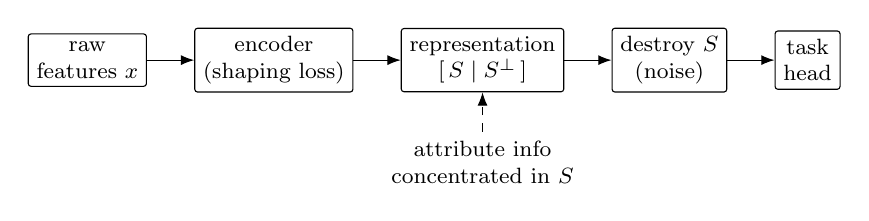
\begin{tikzpicture}[font=\footnotesize, node distance=4mm and 6mm,
  box/.style={draw, rounded corners=1pt, align=center, inner sep=3pt, minimum height=6mm}]
\node[box] (x) {raw\\features $x$};
\node[box, right=of x] (enc) {encoder\\(shaping loss)};
\node[box, right=of enc, minimum width=17mm] (rep) {representation\\$[\,S \mid S^{\perp}\,]$};
\node[box, right=of rep] (noise) {destroy $S$\\(noise)};
\node[box, right=of noise] (head) {task\\head};
\draw[-{Latex}] (x) -- (enc);
\draw[-{Latex}] (enc) -- (rep);
\draw[-{Latex}] (rep) -- (noise);
\draw[-{Latex}] (noise) -- (head);
\node[below=5mm of rep, align=center] (att) {attribute info\\concentrated in $S$};
\draw[-{Latex}, dashed] (att) -- (rep);
\end{tikzpicture}
\caption{% TODO(Nathan): refine schematic + caption.
Shape-then-destroy. Training concentrates attribute information into subspace $S$; $S$ is destroyed with noise before the task head. Ablations show both halves are necessary.}
\label{fig:schematic}
\end{figure}

\begin{figure}[t]
\centering
\figorbox{figures/fig4_two_tier.pdf}{\columnwidth}
\caption{Utility kept at the certified operating point of the end-to-end
noised channel, per cell and per tier (error bars: spread over three
training seeds). Tier~1 (black box) is nearly free where the diagnostic
predicts removal is achievable, and what remains exposed afterward is
only the output-level floor, which is fundamental. Tier~2 (adding the
informed likelihood-ratio attacker) is bought only by more full-rank
noise, at $\sigma{=}20$/$24$/$64$, and its price is the visible drop. On
the hard cell the diagnostic predicts no useful certified point exists,
and none does.}
\label{fig:twotier}
\end{figure}

\section{The Gauntlet: Published Methods Under Identical Evaluation}

We ran the field's published fair-representation and erasure methods
through the identical two-tier battery on the three headline cells, with
knob sweeps, best honest operating point per tier, and three-seed
certification. Each row carries a provenance tag (official code,
validated reimplementation, or generic mechanism), summarized in
Table~\ref{tab:gauntlet} with per-baseline detail in the appendix. One of
36 method--cell--tier combinations certifies.

\textbf{VFAE} \citep{louizos2016vfae} is the one survivor, and it
certifies through its accidental sampling noise rather than its fairness
machinery. The sampled-$z$ exposure holds Tier~1 on the easy cell at
$0.535$ with $72\%$ utility. The posterior-mean exposure of the same
models reads $1.00$ at every $\beta$, and raising the fairness knob makes
sampled-$z$ recovery strictly worse, $0.536$, $0.583$, $0.661$, $0.743$
for $\beta = 1, 10, 10^2, 10^3$, because a larger MMD weight shrinks the
posterior noise faster than it matches groups. Its Tier-2 reading of
$0.551$--$0.556$ is at the bar, not under it, and with no noise knob it
fails the middle and hard cells at $0.585$ and $0.587$. It is the
exception that proves the mechanism: the only baseline that certifies
anything does so exactly where the diagnostic says removal is cheap, via
an unadjustable noise channel it does not control.

\textbf{Obliviator} \citep{akbari2025obliviator}, run from the authors'
pinned official code in its strongest supervised mode, fails Tier~1 on
all three cells at every one of its 15 iterations, reading
$0.968$--$0.999$ while keeping $85$--$99\%$ utility, and its own MLP
stopping probe reads $0.94$--$0.99$ throughout, so its termination
criterion never fires. This matches the prediction of our controlled
HSIC projections (Fig.~\ref{fig:demolition}): on representations where
the attribute is robustly and nonlinearly encoded, HSIC-guided erasure
has almost nothing kernel-visible left to remove, however seriously it
is engineered.

\textbf{LAFTR} \citep{madras2018laftr}, both as our validated multiclass
reimplementation and re-run on the official Vector Institute release
under a compatibility shim calibrated to the paper's own Adult numbers,
fails Tier~1 everywhere, at $0.846$--$1.000$ across every adversary
weight. The official run adds one diagnosis: at $\gamma \ge 2$ on the
easy cell the min-max ``wins'' fairness by zeroing task utility, lift
falls to $3$--$17\%$ of clean, while the representation still leaks at
$0.996$--$1.000$. \textbf{DANN-style adversarial scrubbing}
\citep{ganin2015dann}, our generic-mechanism baseline at full strength,
genuinely removes signal but plateaus at $0.610$--$0.664$ for
$42$--$69\%$ utility. \textbf{LEACE} \citep{belrose2023leace}, from the
authors' library, reads $0.995$--$0.998$ at nearly full utility, the
unprotected level, as its linear scope predicts on representations that
encode the attribute nonlinearly. In plain terms, no published method
reaches the purpose-built channel on any cell at either tier, and the
single certifying combination is an accident of a stochastic encoder.

\begin{table}[t]
\centering
\footnotesize
% TODO(Nathan): numbers below are from the final gauntlet report; verify each
% against results/baseline_gauntlet.json before submission. Consider moving
% per-cell detail to appendix and keeping the verdict summary here.
\begin{tabular}{@{}lllcc@{}}
\toprule
Method & Provenance & Utility & T1 & T2 \\
\midrule
LAFTR & official+calib. & -- & \texttt{0.995+} & fail \\
VFAE & valid.\ reimpl. & 72\% & \textbf{pass}$^{1}$ & at bar \\
DANN-scrub & generic mech. & $\le$58\% lost & fail & fail \\
LEACE & official pkg. & -- & \texttt{0.995+} & fail \\
Obliviator & official (N'25) & -- & \texttt{0.97+} & fail \\
\midrule
Ours (post-hoc) & this work & 53--89\% & pass & fail \\
Ours (e2e) & this work & 85--102\% & \textbf{pass} & pass$^{2}$ \\
\bottomrule
\end{tabular}
\caption{% TODO(Nathan): finalize columns/footnotes.
Gauntlet summary across the three headline cells and two threat tiers; 1 of 36 published-baseline combinations certifies. $^{1}$Easy cell only, via incidental sampling noise. $^{2}$Tier-2 certification via full-rank noise at the costs of Fig.~\ref{fig:twotier}.}
\label{tab:gauntlet}
\end{table}

\section{Discussion}
% TODO: ~0.3pp.
% - Way 1 as finding (if not already in the law section): the floor is
%   label-relative; measured walls may partly reflect label bias.
% - Limitations, honestly: tabular + one vision check; the diagnostic's validity
%   condition; 0.55 is a chosen bar; Tier-2 achievability is expensive.
% - Future work: 2-3 sentences on prevention vs removal for entangled capabilities
%   in language models (Way 3, do not spend it); 1 sentence on output-level
%   mechanisms such as differentially private responses (Way 4).
[Discussion stub.]

\bibliography{references}

% =====================================================================
% APPENDIX MATERIAL BELOW. At submission this moves to the separate
% supplementary file per AAAI instructions. Kept here during drafting.
% =====================================================================
% \appendix
% \section{Proofs}            % Prop 1 (half page); Prop 2 (construction + computed instance)
% \section{CelebA Details}    % both cells, the reconciliation, scope note on pre-shaped reps
% \section{Provenance}        % per-baseline provenance + deviations tables
% \section{Per-Baseline Analyses} % LAFTR knob sweep, VFAE variants, Obliviator iterations
% \section{Reproducibility}   % pointer to anonymized repo; checklist filed separately

\end{document}
